\documentclass[acmtog,review]{acmart}

\usepackage{booktabs} % For formal tables

\acmPrice{15.00}
\settopmatter{authorsperrow=4}

\usepackage[utf8]{inputenc}

\usepackage{hyperref}
\usepackage{xcolor}
\usepackage{subcaption}
\usepackage{amsmath}
\usepackage{algorithm}
\usepackage{graphicx}
\usepackage{algorithmic}


\usepackage{todonotes}

\usepackage{enumitem}

\hypersetup{
colorlinks=true,
linkcolor=red,
citecolor=green,
filecolor=magenta,
urlcolor=cyan
}

\DeclareMathOperator*{\argmax}{arg\,max}
\DeclareMathOperator*{\argmin}{arg\,min}

\begin{document}

\title{U2F HID Implementation - Microprocessor to U2F Key}
\subtitle{6.858 - Computer Systems Security. May 5th, 2022.}

% Authors.
\author{Torque (Tareq) El Dandachi}
% \affiliation{
% \department{EECS and MechE}
% \institution{MIT}}
\email{tareqdandachi@gmail.com}

\author{Ashika Verma}
\email{ashikav@mit.edu}

\author{Muhammad Abdullah}

% This command defines the author string for running heads.
% \renewcommand{\shortauthors}{DeJohnette, Rowland-Smith, Badeeri, and Foyt}
\renewcommand{\shortauthors}{Torque (Tareq) El Dandachi, Ashika Verma, Muhammad Abdullah}
\settopmatter{printacmref=false}

\renewcommand\footnotetextcopyrightpermission[1]{} % removes footnote with conference information in first column
\pagestyle{plain} % removes running headers
\fancyfoot{}

\makeatletter
\let\@authorsaddresses\@empty
\makeatother


% abstract
\begin{abstract}
We design and implement a U2F Key that follows the FIDO2 U2F Protocol. The key is
designed to interact with WebAuthn across different browsers as a second factor
authenticator device. The \href{https://github.com/tareqdandachi/u2f}{code} is 
designed to be uploaded onto a teensy with one button for verifying user presence.
We use two AES128 encrypted keys hard-coded upon installation, $K_{wrap}$ and $K_{app}$ to generate the handle and encrypt the application parameter.
% \todo[inline]{abdullah describe our encryption DONE}
\end{abstract}

%keywords
% \keywords{U2F, FIDO2, }

\maketitle
\thispagestyle{empty}

\section{Introduction}
 
\subsection{Overview of U2F}
Universal 2nd Factor (U2F) is an open standard that strengthens and simplifies two-factor authentication using specialized USB or NFC devices based on similar security technology found in smart cards. Essentially, it adds a second layer of protection to the simple username and password that many web services employ. The user flow of trying to log in remains similar: a user logs in with their username and password. However, at any point in time, the web service can request the user for their second factor for authentication. 

For our project, we designed and implemented a U2F Key which follows the FIDO2 U2F protocol. In the following sections, we explain how we implemented and interacted with each component of the protocol, including encryption, the hardware we used for the security key, communication between the hardware and client, web authentication, and future steps.
 
\subsection{GitHub Repository}
All of our code can be found in our GitHub repository, \\ \hyperlink{https://github.com/tareqdandachi/u2f}{github.com/tareqdandachi/u2f}. We include code which implements the U2F protocol for a Teensy 3.2 to create a security key, and code to create a website which uses the U2F protocol for credentials.

\subsection{FIDO2 U2F}
We focused on implementing the FIDO2 U2F protocol. For FIDO2 U2F, the user must present a security key for their second factor, which is usually a USB device. There are two flows in the FIDO2 U2F protocol, registration and authentication as show in Figure \ref{reg} and \ref{auth}.

\addtocounter{footnote}{1}
\footnotetext{Figures copied from \url{https://css.csail.mit.edu/6.858/2022/readings/u2f-fc.pdf}}

\begin{figure}
  \caption{Security Key Registration$^1$}
  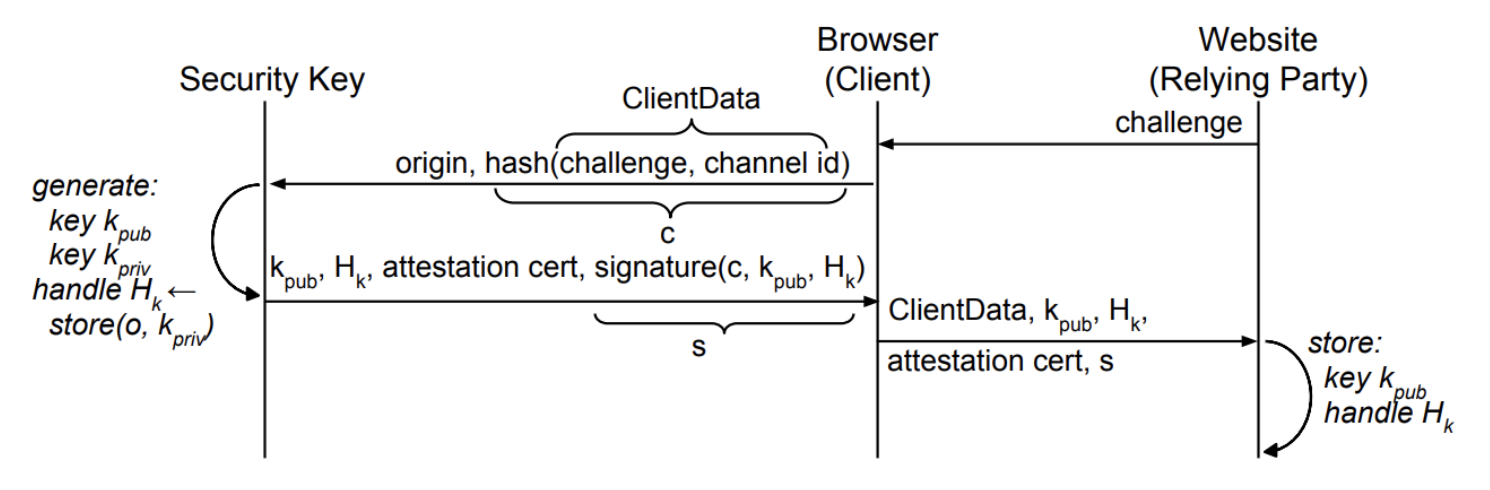
\includegraphics[scale=0.35]{register.png}
  \label{reg}
\end{figure}

\begin{figure}
  \caption{Security Key Authentication$^1$}
  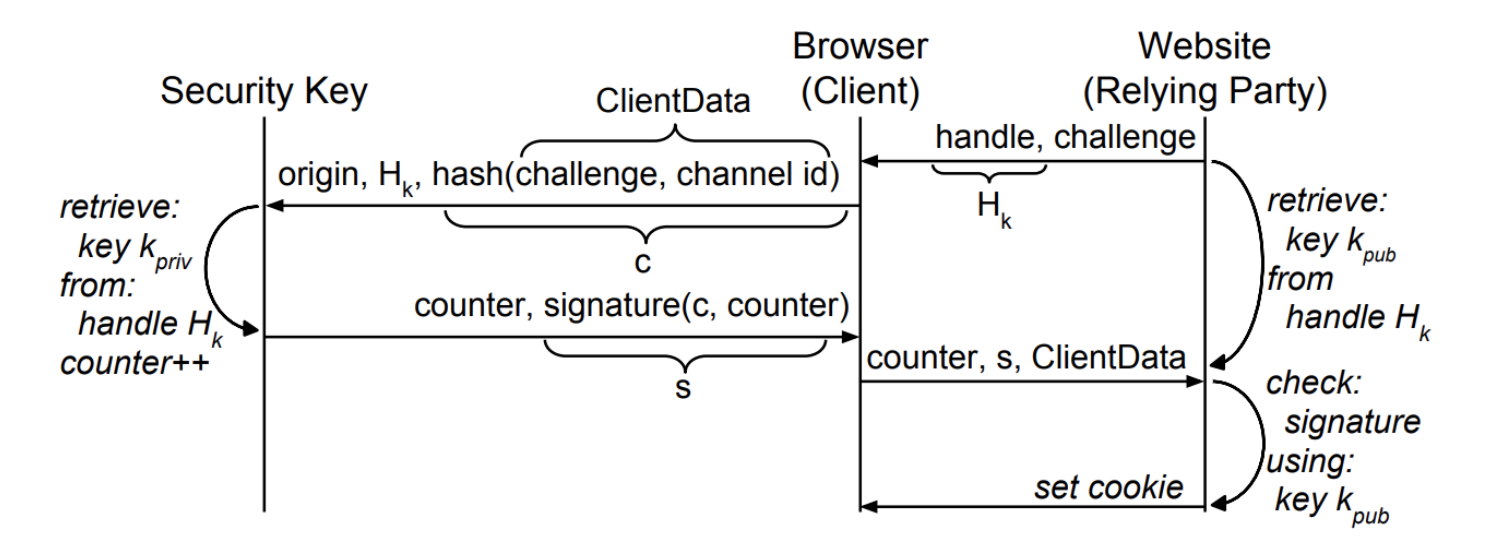
\includegraphics[scale=0.35]{authenticate.png}
  \label{auth}
\end{figure}

There are three different components to make the U2F protocol secure, the website (or relying 
party), the user's browser (client), and the security key. Registration and authentication 
are a three step process: (1) the relying party issues a challenge to the security key, 
(2) the security key signs the challenge, and (3) the relying party checks the signature 
with the security key's public key. To prevent against Man-in-the-Middle (MitM) attacks, 
the origin and TLS channel ID are hashed and passed along as the application parameter to the security 
key, is then signed by the security key, which when passed back to the relying party, and can be verified using the public key send during registration. To prevent against device 
cloning attacks, the security key has a counter which increments while authenticating and is forwarded to the client. If the counter is ever less than the counter the relying party
stored, then the security key has been compromised.
Lastly, there's an attestation
certificate which can be re-used in multiple keys allowing clients to revoke keys if a certain model is compromised or it can be used for added checks 
such as a banking website only wanting their own signed security keys to be used on their website.


\section{U2F Protocol}
\label{u2f_protocol}
% \todo[inline]{abd}

\subsection{Request Message Framing}

The U2F Request message is framed in a standard application protocol data unit (APDU) format. This requires a 7-byte header in the following order:

\begin{itemize}
    \item \textbf{CLA}: Always 0x00.
    \item \textbf{INS}: The instruction to be executed.
    \item \textbf{P1-2}: Two parameter bytes, \textbf{P1} and \textbf{P2}.
    \item \textbf{L1-2}: Length of the data to be transferred.
    \item \textbf{Data}: The request data.
\end{itemize}

The \textbf{INS} header byte determines whether the request is for \texttt{0x01:} \texttt{U2F\_REGISTER}, \texttt{0x02: U2F\_AUTHENTICATE}, \texttt{0x03: U2F\_VERSION} or vendor specific instructions that live between \texttt{0x40 $\xrightarrow[]{}$ 0xbf}
. 
For \texttt{U2F\_REGISTER}, the \textbf{P1} and \textbf{P2} fields are not used. 
Meanwhile  \textbf{P1} field is used by the FIDO Client for \texttt{U2F\_AUTHENTICATE} to specify between 
\textbf{check-only} authentication (\texttt{0x07}) or \textbf{enforce-user-presence-and-sign} authentication (\texttt{0x03}).
\subsection{Processing Registration Requests}

For registration, the request data is 64 bytes long. The first 32 bytes are the challenge hash followed by the application parameter.
Following the U2F Protocol, the U2F key generates a key pair and a handle from \texttt{store(application parameter, private key)}.
It also generates a signature and appends it to the end.

The data is first hashed with SHA-256 and then signed with the attestation key belonging to the attestation certificate.
The response is constructed as follows: \\

\begin{figure}[H]
    \centering
    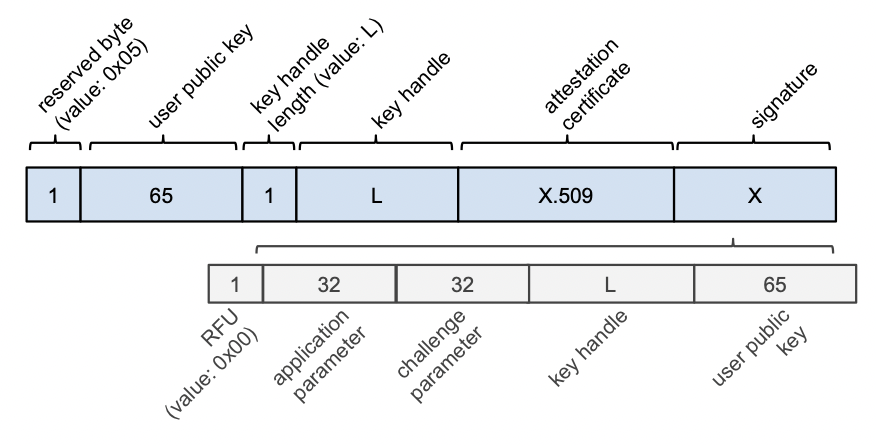
\includegraphics[scale=0.5]{regresp}
    \caption{Framing of a successful registration response$^2$}
\end{figure}

\addtocounter{footnote}{1}
\footnotetext{Figures copied from \url{https://fidoalliance.org/specs/fido-u2f-v1.0-ps-20141009/fido-u2f-raw-message-formats-ps-20141009.pdf}}

%\begin{itemize}
%    \item \textbf{Reserved}: Always 0x05.
%    \item \textbf{Public Key}: The uncompressed public key generated by the U2F key. This is a 65-byte array, with the first byte being 0x04 to indicate the public key is uncompressed. The remaining 64 bytes are the public key.
%    \item \textbf{Handle Length}: The length of the handle. This is a single byte.
%    \item \textbf{Handle}: The handle generated by the U2F key.
%    \item \textbf{Attestation Certificate}: The attestation certificate of the U2F key. In X.509 DER format.
%    \item \textbf{Signature}: The signature discussed above, in X.509 DER format.
%\end{itemize}

The certificate and the signature are sent in DER format, the certificate allows the FIDO client to recognise a batch of keys
so that any defective keys can be refused. The exact DER format of the signature is specified in the next section, along with the encryption used in \texttt{store} and \texttt{retrieve}.


\subsection{Processing Authentication Requests}

For authentication, the first 64 bytes of the request data are the challenge hash and the application parameter. This is followed by a byte specifying the key handle length and the key handle.


If the \textbf{P1} field is 0x07, we only need to verify the handle. In that case we use a modified \texttt{retrieve} operation as defined in Alg. \ref{alg:retrieve}. 
We do not return the private key, instead the return value is conditional on the assertion \texttt{app'' == app'}.
If the assertion passes, we respond with the error message ``Test-of-user-presence required'': this is the success message for \textbf{check-only} authentication, despite it being an error message in \textbf{P1}\texttt{=0x03}.
If the assertion fails, we respond with the error message ``Bad Key Handle''.
\begin{figure}[H]
    \centering
    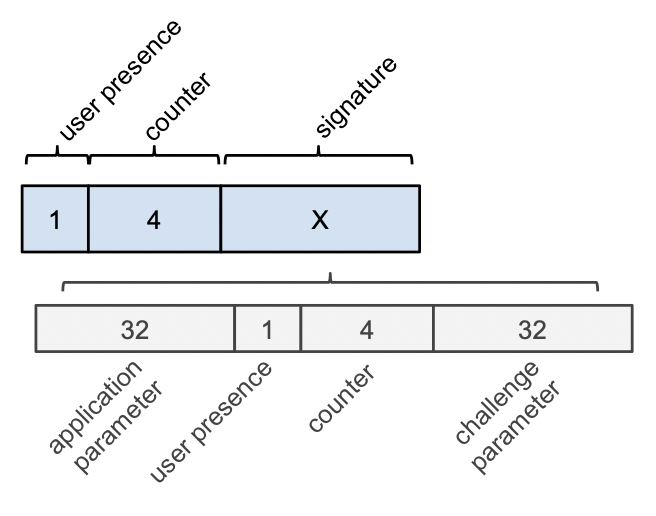
\includegraphics[scale=0.43]{authresp.png}
    \caption{Framing of a successful authentication response$^2$}
\end{figure}

If the \textbf{P1} field is 0x03, we need to verify the handle and the user presence. We then follow the standard U2F authentication process; test for user presence, increment the counter and return the response in the format above. The important difference between this signature and the one used in registration is that this the signature is signed with the private key, not the attestation key.

% I took this out cuz this is my section :p
% \subsection{Response Message Framing}


% The response is also sent in the APDU format. The response is framed in the following order; the response data (constructed
% in the previous sections) | \textbf{SW1} | \textbf{SW2}. The \textbf{SW} bytes are the response status words defined by ISO7816-4, which can take three values in U2F:

% \begin{itemize}
%     \item \textbf{SW\_NO\_ERROR}: Success.
%     \item \textbf{SW\_CONDITIONS\_NOT\_SATISFIED}: User presence not verified.
%     \item \textbf{SW\_WRONG\_DATA}: Bad key handle.
% \end{itemize}


\subsection{Version Requests}

The last type of request is a \texttt{0x03: U2F\_VERSION} instruction request. The response message's raw representation is the ASCII representation of the string \texttt{U2F\_V2}. The command takes no flags.


\section{Encryption}
% \todo[inline]{abd}

% \begin{itemize}
%   \item TRNG seeding - DONE
% 	\item You need to sign deterministically -DONE
% 	\item Our handle is always 64 bytes long bc aes128 - DONE IN INTRO
% 	\item Signature needs to be in DER format - DONE
% 	\item We drop the last byte of the DER certificate (I don’t know why we do that) - DONE
% \end{itemize}

\subsection{True RNG}

We seed the key generation with static to get better entropy. This is done by reading analog pin $0$ and taking the least 
significant bit of the result. If the result doesn't change between two reads, then we count the number of cycles
it takes to change and use the count's least significant bit as the next bit. 

\subsection{Signature}

The signature is done deterministically using the relevant key. The DER format requires that the signature
data (R,S pair) is appended in the following order:

\begin{itemize}
    \item \textbf{Header}: 0x30 for compound structure.
    \item \textbf{Length}: The length of all that follows 
    \item \textbf{Header}: 0x02
    \item \textbf{Length}: The length of the R-value.
    \item \textbf{R-Value}: The R-value.
    \item \textbf{Header}: 0x02
    \item \textbf{Length}: The length of the S-value.
    \item \textbf{S-Value}: The S-value.
\end{itemize}

We also drop the last byte of the attestation certificate.

\subsection{Handle Encryption}

We use the specification described in the original U2F paper for store and retrieve.

\begin{algorithm}
    \caption{Store(app, $k_{priv}$) $\rightarrow$ H}
    \label{alg:store}
    \begin{algorithmic}
        \STATE $app' \leftarrow Encrypt(app)_{K_{app}}$
        \STATE $plaintext \leftarrow Interleave(k_{priv},app')$
        \STATE $H \leftarrow Encrypt(plaintext)_{K_{wrap}}$
        \RETURN $H$
    \end{algorithmic}
\end{algorithm}

\begin{algorithm}
    \caption{Retrieve(app, H) $\rightarrow$ $k_{priv}$ }
    \label{alg:retrieve}
    \begin{algorithmic}
        \STATE $app' \leftarrow Encrypt(app)_{K_{app}}$
        \STATE $plaintext \leftarrow Decrypt(H)_{K_{wrap}}$
        \STATE $(k_{priv},app'') \leftarrow Deinterleave(plaintext)$
        \STATE assert $app' == app''$
        \RETURN $k_{priv}$
    \end{algorithmic}
\end{algorithm}


The encrypt and decrypt functions use AES-128 in 16-byte blocks on the 32 or 64 byte data, done using the Electronic Code Book (ECB) scheme. ECB is simpler than the standard Cipher-Block Chaining scheme at the cost of unreliable obfuscation on large plaintext with patterns. That is not an issue in our case since we encrypt at most 4 blocks of data alongside interleaving which further reduces detectable patterns.

\section{Hardware}

\subsection{Microcontroller}
\label{Microcontroller}

We developed and tested this implementation on a Teensy 3.2. We 
based this on 3 main factors:

\begin{enumerate}
    \item The Teensy 3.2 has a built-in EEPROM memory we can use to store the counter that
    retains memory even when shut off.
    \item It is capable of full-speed HID communication using RawHID which is used to send 64 bytes 
    per packet.
    \item It is small and has accessible solder pads to add our own connections to the USB
    power and data bus.
\end{enumerate}

To use the microcontroller as an HID device that interacts with WebAuthn, we need it
to be discoverable as a FIDO device. This identification is done by defining a
control usage defined by changing the usage page and usage id parameters of
our device. The FIDO standard requires our usage page to be defined as \texttt{0xF1D0}
and usage id as \texttt{0x01}. These can be changed by modifying the \texttt{usb\_desc.h}
file that corresponds to the RawHID protocol in the \texttt{teensy3} source.

\subsection{Physical Key with Button}

For our physical device, we designed a small key with a male USB A port and a button for verifying 
user presence. The button is in a pull down configuration with the electronics placed on a 
protoboard that is soldered onto the teensy body. 
The button is connected to pin 19 on the microcontroller.
We soldered the male USB A port
onto the solder pads below the teensy 3.2 corresponding to $D+$, $D-$, power and ground.
The device we ended up making is displayed in figure \ref{fig:device}.

\begin{figure}
    \centering
    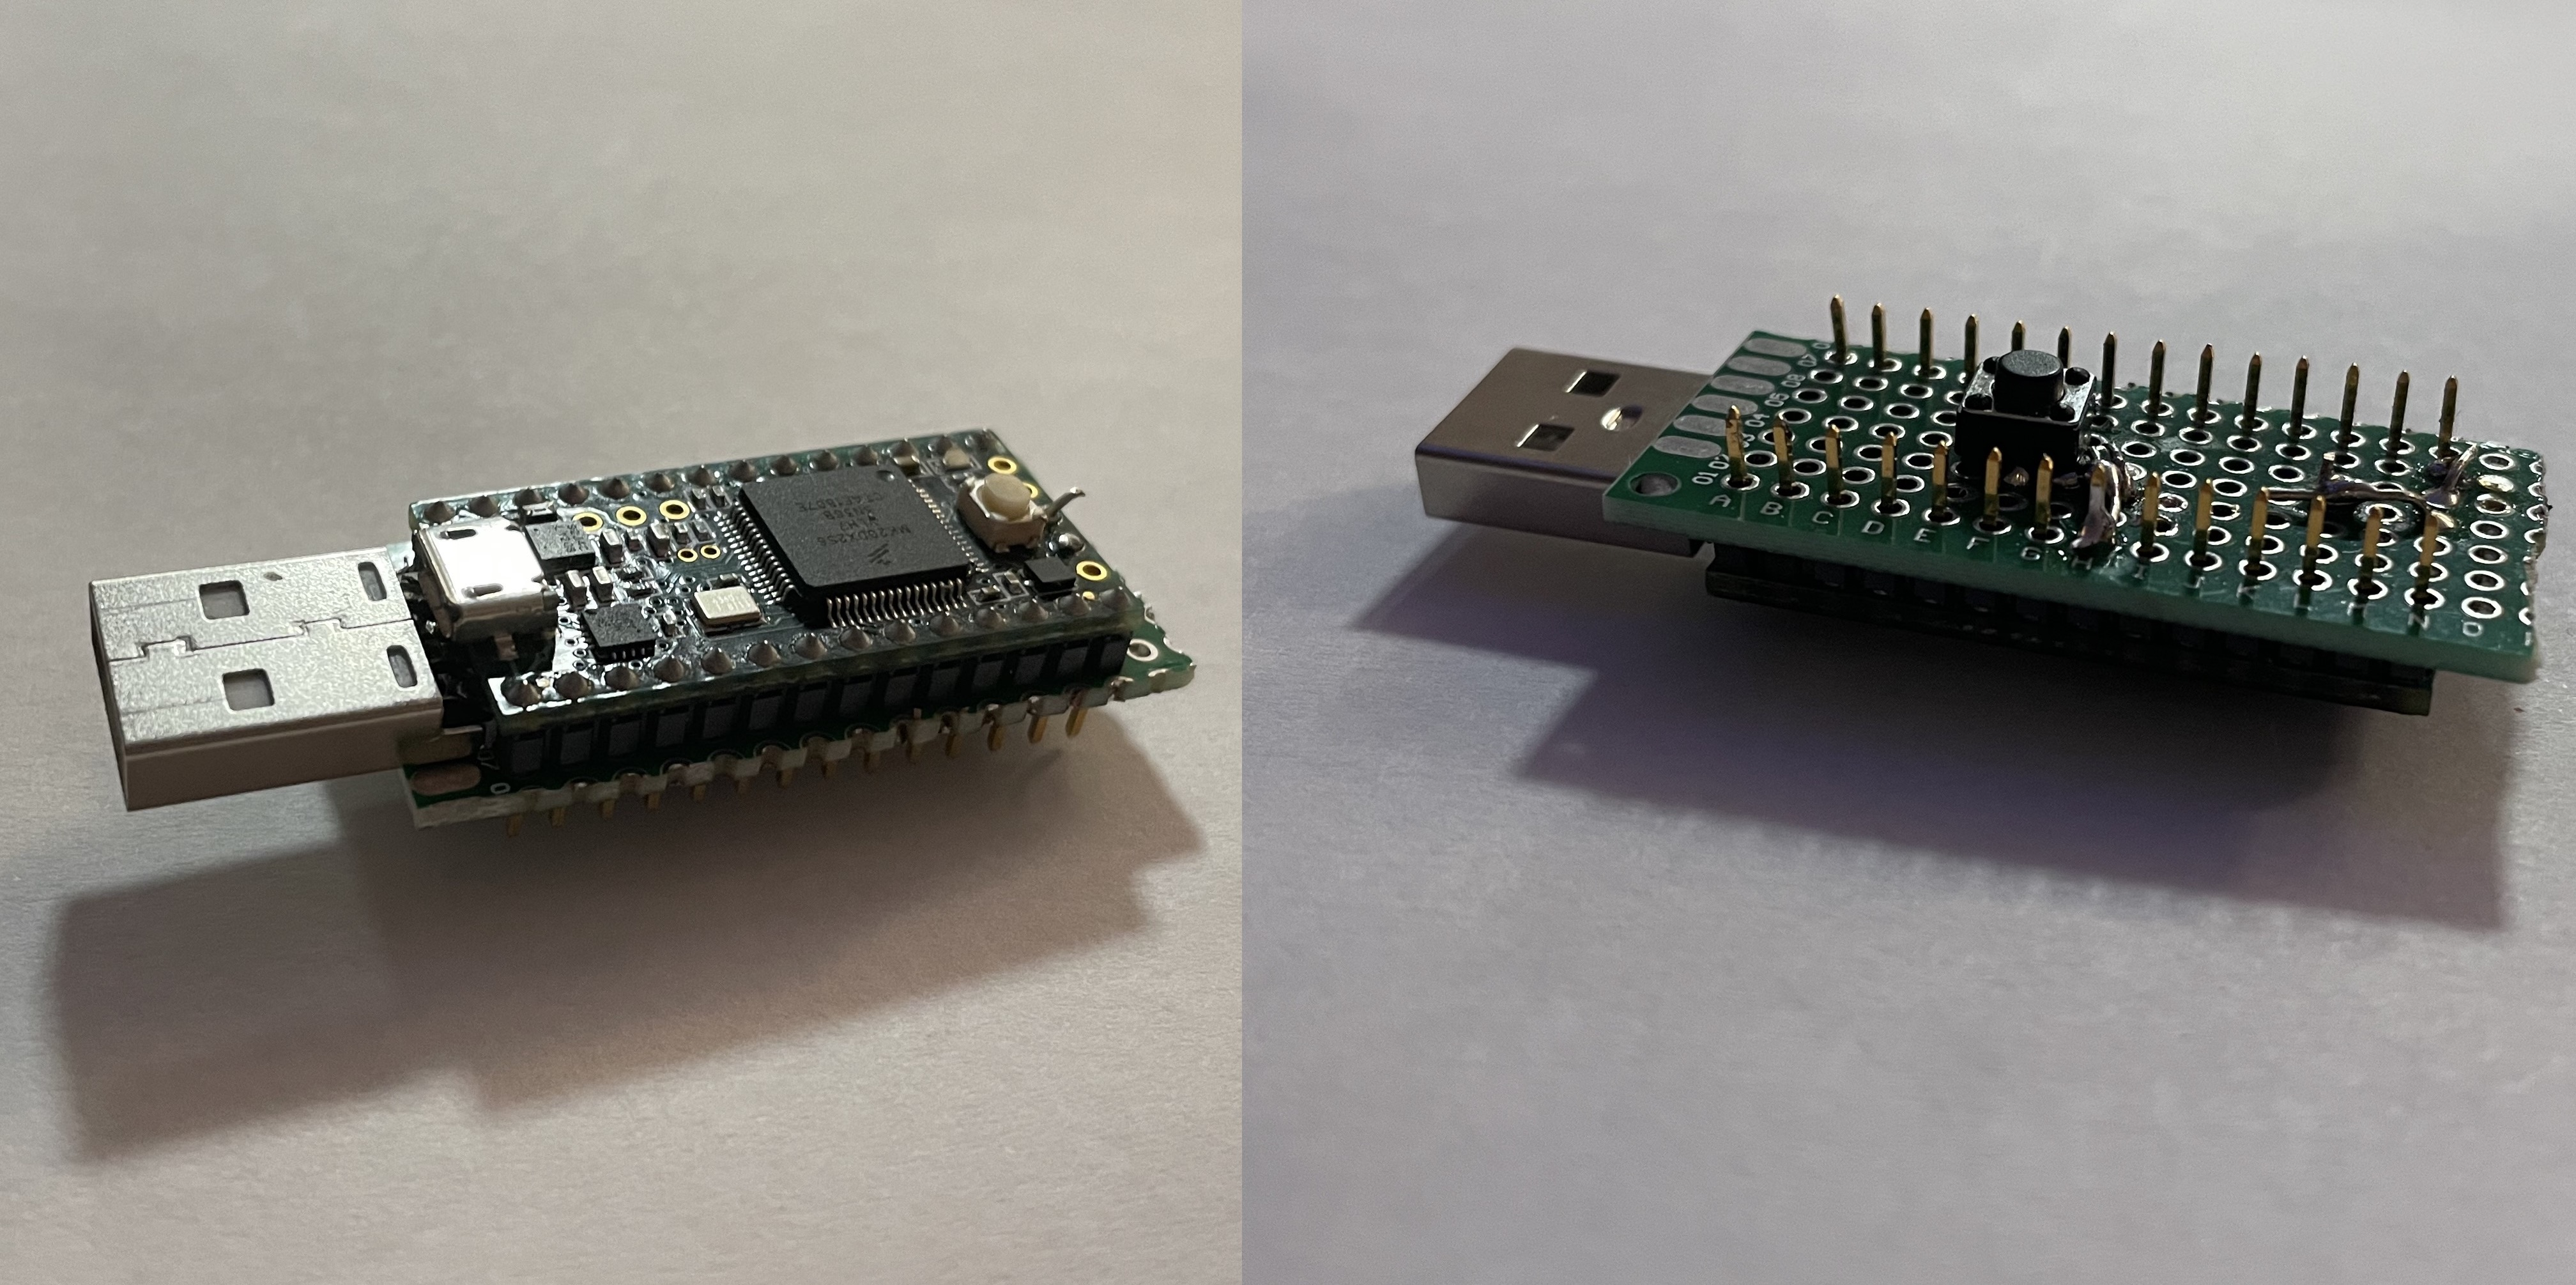
\includegraphics[width=3.2in]{hardware_key.jpeg}
    \caption{Teensy 3.2 with both a male USB A port and a female micro-USB B port. The teensy has a protoboard attached to one side that houses a button and a $1$K resistor in a pull down configuration.}
    \label{fig:device}
\end{figure}



\section{Communication}
\label{comm}

\subsection{RawHID and U2FHID}

For robust bidirectional communication with USB host applications, we use 
RawHID. We implement the FIDO2 U2F protocol over USB HID (Human Interface Device)\footnote{\url{https://fidoalliance.org/specs/fido-u2f-v1.2-ps-20170411/fido-u2f-hid-protocol-v1.2-ps-20170411.pdf}}.
HID transfers use smaller data chunks per transaction and don't require drivers
causing them to be more reliable than USB CDC (Communications Device Class) 
transfers (i.e. virtual serial ports).

Our hardware supports sending and recieving 64-byte packets with a host application,
in this case a WebAuthn client. Since it doesn't require drivers, it works out of the
box and should automatically be detected by browsers that implement the WebAuthn API.
This transfer method allows for multi-application support, fixed latency and low-overhead;
making the U2FHID protocol much more scalable for discovery and use.
When the HID communication begins, our hardware sends parameters over that specify
the vendor id, product id, usage page and usage id (discussed in section \ref{Microcontroller}).

Messaging in this protocol consists of three layers. Firstly, we need a way to carry
HID reports at the channel level and encode messages inside of these transactions. 
This level of messaging contains instructions that start, end and communicate within the HID scheme. They are also responsible for channel allocation and propagating errors at the HID level. The second layer
focuses on Application Protocol Data Unit (APDU), a way to encode response and request
data along with status words. The final layer deals with the representation of response
and request data in a way pertaining to our protocol, this is discussed in section \ref{u2f_protocol}.


\subsection{Communication Protocol/Transactions}

\subsection{Packets and Channels}

The U2FHID protocol defines transactions, which are requests followed by a message.
Transactions are blocking once intiated: once a transaction is initiated, it needs 
to be fully resolved before a new transaction takes place. Messaging is done through
a smaller unit of data called a packet, these correspond to HID reports. Packets have
a fixed size.

The protocol is designed for concurrency: multiple clients can access a single resource
through the HID stack. The protocol defines logical channels (channels handled through
encoding rather than physically different channels). To manage routing, our implementation
assigns one of four unique channel identifiers to each application. Channel identifiers
are 32-bit numbers where \texttt{0x00000000} and \texttt{0xffffffff} are reserved. 
\texttt{0xffffffff} is used for channel allocation.

To manage concurrency, we keep track of 5 internal states: \\\texttt{Available}, 
\texttt{Wait\_init}, \texttt{Wait\_cont}, \texttt{Timeout}, \texttt{Large}. This helps
our device manage concurrency with requests, enter busy modes and allow for consistency
between the processing requests.

\subsection{Messaging and Headers}

Each request and response begins with an initialization packet and is followed by 
continuation packets if the messaging requires more space. The U2F device never sends
a response if no request is initiated from a host.

\subsubsection{Initialization Packets}

The first 32 bits of all packets are a channel identifier. Next follows 8 bits
corresponding to a command identifier. The command identifier encodes different U2FHID 
commands such as \texttt{U2FHID\_MSG}, \texttt{U2FHID\_INIT} and \texttt{U2FHID\_ERROR}. 
The next 16 bits encode the payload length. The remaining
57 bytes are the payload. The command identifier always ahs the highest bit set to
1 (command identifier always greater than \texttt{0x7f}), to distinguish it from
a continuation packet which has that bit always set to 0.

\subsubsection{Continuation Packets} As with initialization packets, the first 32 bits
encode the channel identifier. This is followed by a bit that is always set to zero,
identifying the packet as a continuation packet. 
The next 7 bits encode the packet sequence which starts at 0 and is incremented for
every next packet. This is then followed by 59 bits corresponding to the payload.
Note that this means with our implementation of 64-bytes of HID communication
(the maximum for full-speed devices), the maximum payload length is 7609 bytes.

\subsection{Message Framing}

\subsubsection{Request Message APDU}

The request message is encoded using the Application Protocol Data Unit (APDU) spec
and needs to be processed to extract the different parts of it. The APDU can be
encoded in 
Extended Length Encoding for a maximum length of 65,535 bytes or a Short Encoding
allowing a maximum of 256 bytes to be sent. 
The message payload is prefaced with a CLA byte which we set and check to be zero.
It is then followed by an instruction code which contains U2F protocol instruction
codes that specify what part of the U2F protocol to run. This is followed by 2 parameters
defined by the U2F instruction used. It is followed by the length of the request data and 
expected length of the payload.

\subsubsection{Response Message APDU}

The response message ADPU contains the response data followed by a 16-bit status word.
The U2F protocol defines 6 status words as defined in ISO7816-4 with a special meaning:
\begin{enumerate}
    \item \texttt{0x9000 SW\_NO\_ERROR}: command completed successfully.
    \item \texttt{0x6985 SW\_CONDITIONS\_NOT\_SATISFIED}: failed test of user presence.
    \item \texttt{0x6A80 SW\_WRONG\_DATA}: invalid key handle.
    \item \texttt{0x9000 SW\_WRONG\_LENGTH}: invalid length of request.
    \item \texttt{0x6E00 SW\_CLA\_NOT\_SUPPORTED}: ``Class byte of the request is not supported.'' In our implementation, CLA byte is enforced to be \texttt{0x00}.
    \item \texttt{0x6D00 SW\_WRONG\_LENGTH}: requested instruction not supported, our implementation only supports the main 3 outlined in the U2F spec with no other vendor specific instructions: \texttt{U2F\_VERSION}, \texttt{U2F\_REGISTER} and \texttt{U2F\_AUTHENTICATE}.
\end{enumerate}



% \subsection{Error handling}

% \todo[]{DO WE WANT THIS?}

\section{WebAuthn}
% yeehaw LOL 
% heyhey hi:) is WebAuthn a library? I sent a msg on messenger
% I am a lil confused what to call it since, did u like import WebAuthn or how does it work lol
% it's an API so WebAuthn is short for webauthenticaion api
% lol
% hmmm. So what is chrome communication part of? The API? Chrome ?->? USB
% Maybe a better question is what did u import or where are the functions u call defined in?


% https://www.w3.org/TR/WebAuthn-2/#sctn-api
% also i didn't import anything, its just there to use it's kinda wack
% navigator.credentials.create()
% navigator.credentials.{use any method here}
% What is the function name?
% https://developer.mozilla.org/en-US/docs/Web/API/Navigator/credentials
% the browsers just have them - thats crazy
% lmfao nerd

% HOW DARE :((( 
% <3
% Also maybe mention this in the intro/WebAuthn section, thats p cool. didnt know W3C was part of it :)))):


% hi bestie - what does mention all devices recv req, first presence return 
% mean?
% and also screening by usage page and id
% lmfao
% gotcha
% hello! ummmm So it turns out WebAuthn sends a request transaction to all devices
% connected - so if u have 5 keys all of them get the request. Then the first one
% to get user presence is the one that sends a response and I think the rest just are ignored.
% ooh okey! tyty
% For screening usage page and id. Every HID protocol screens devices talking to it based on
% usage page and usage id. These r the registers I modified and I talk about it. But mention that
% the WebAuthn screens for things with usage page \texttt{0xf1d0}.

% \todo[inline]{ash, maybe move section before communicartion?}

\subsection{WebAuthn API}
The Web Authentication API (WebAuthn) is a specification written by W3C and FIDO with participation of Google, Mozilla, Microsoft, Yubico and others. It is a public key extension of the existing credential management API. Essentially, it allows servers to register and authenticate users using the FIDO2 U2F framework and makes it easy for servers to add this additional layer of security to the servers current password management system. In addition to the supporting FIDO U2F devices, WebAuthn also allows other types of authenticators such as Android Attestation Keys or Trusted Platform keys (like the fingerprint sensor on some MacBooks).

\subsection{Registration}
The client first issues a request to the relying party to register along with user information for the relying party to store credential information about the user. Next, using WebAuthn, the relying party can issue a 32 byte challenge and pass along parameters such as relying party url or the type of attestation. From there the browser issues requests for a second factor to register. The user can press their FIDO-U2F compliant security key to run through the protocol detailed in Section 2. 
The Webauthn API creates a \texttt{PublicKeyCredential} object which contains the \texttt{ClientData} (challenge and origin) and attestation object (signature, public key, and handle). The client then send the \texttt{PublicKeyCredential} to the relying party or server. The \texttt{PublicKeyCredential} can be decoded and unravelled to get the \texttt{ClientData}, public key of the security key, the handle, the attestation certificate and signature, which the relying party uses as shown in Figure \ref{reg}. The relying party can check the signature with the public key and if needed verify the attestation certificate. The relying party then stores the public key of the security key and handle in its own database. From there, the relying party can tie a user to these new credentials by saving these credentials.

\subsection{Authentication}
Authentication follows a similar flow as registration using Webauthn, except the security key sends back a counter and a signature of the counter plus the hash of the \texttt{ClientData}. The relying party then checks the signature with the private key that it stored earlier and also checks if the counter has increased from the previous observed value to prevent device replication attacks. After authentication, the relying party can log the user in for the rest of the session.

\subsection{WebAuthn Requests}

The WebAuthn API communicates with keys using requests as discussed in section \ref{comm}. 
Once a host triggers a WebAuthn authenticate message, the message is broadcast to all
connected U2F devices. The first device to respond with a positive test of user presence
allows the authenticator to continue with the communication. The broadcast to all
connected U2F devices is filtered by the usage page that corresponds to that of the FIDO2 
U2F protocol as discussed in \ref{Microcontroller}.

\subsection{Testing HID to WebAuthn Communication}
We created our own relying party which uses WebAuthn which can be accessed at \href{https://u2f-858.herokuapp.com/}{u2f-858.herokuapp.com}. However, other useful
resources to verify the entire stack is functional included:
\begin{itemize}
  \item \href{https://webauthn.io/}{webauthn.io}
  \item \href{https://demo.yubico.com/webauthn-technical/registration}{demo.yubico.com/webauthn-technical}
\end{itemize}

\section{Results and Future Steps}
% \todo[inline]{torq}

Our implementation worked on registering and authenticating on modern websites and
is secure against testing on the Yubico Key testing suite. We published our implementation
onto \href{https://www.github.com/tareqdandachi/u2f}{GitHub}. The implementation works as-is
with little to no hardware modification (the addition of a button for user presence but that
can be turned off).

Given more time, we would like to develop changes on the hardware. Namely, we would want to
add a true random number generator hardware module that we sample from instead of seeding
randomness by measuring static. We would also design hardware specifically for encryption
and decryption on a secure element. We hope to be able to convert this implementation into
robust hardware rather than software running on a microprocessor to remove the reliance
on a secure infrastructure provided by the teensy. 

On the software side of things, we hope to emphasize the accessiblity of this implementation
so that anyone could load this onto any microcontroller they have. We designed and tested this
on a Teensy 3.2, but there is nothing that is completely specific and not reproducible
on other hardware (except for counter on EEPROM on some devices). Hopefully this could
turn into a user friendly program people can use to make a custom key without needing
to install arduino.

\vspace{100px}
\newline
\vspace{10px}
\newline
\vspace{10px}
\newline
\vspace{10px}
\newline
\vspace{10px}
\newline
\vspace{10px}
\newline
\vspace{10px}
\newline
\vspace{10px}
\newline
\vspace{10px}
\newline

% \bibliographystyle{ACM-Reference-Format}
% \bibliography{main}

\section*{References}

\begin{enumerate}
    \item \url{https://fidoalliance.org/specs/fido-u2f-v1.0-ps-20141009/fido-u2f-hid-protocol-ps-20141009.html}
    \item \url{https://fidoalliance.org/specs/fido-u2f-v1.0-ps-20141009/fido-u2f-raw-message-formats-ps-20141009.pdf}
    \item \url{https://fidoalliance.org/specs/fido-u2f-v1.2-ps-20170411/fido-u2f-hid-protocol-v1.2-ps-20170411.pdf}
    \item \url{https://fidoalliance.org/specs/fido-u2f-v1.2-ps-20170411/fido-u2f-raw-message-formats-v1.2-ps-20170411.html}
    \item \url{https://fidoalliance.org/specs/fido-v2.0-id-20180227/fido-client-to-authenticator-protocol-v2.0-id-20180227.html}
    \item \url{https://fidoalliance.org/specifications/}
    \item \url{http://www.linux-usb.org/usb.ids}
    \item \url{https://github.com/tonijukica/webauthn.git}
    \item \url{http://bitcoin.stackexchange.com/questions/12554/why-the-signature-is-always-65-13232-bytes-long}
    \item \url{https://css.csail.mit.edu/6.858/2022/readings/u2f-fc.pdf}
    \item \url{https://demo.yubico.com/webauthn-technical/}
    \item \url{https://webauthn.io/}
\end{enumerate}

\end{document}